%\todo{Talk about other potential PRET applications, and that PRET can be used to more tightly integrate software and hardware.}
In this chapter we will present two applications that have been implemented with our Precision Timed Architecture.
The first application is a real-time one dimensional computational fluid dynamics (1D-CFD) simulator.
This simulator runs in real-time to simulate the fuel rail pressure and flow rate for improved engine efficiently when injecting fuel.
The application makes use of the light weight hardware threads in our thread-interleaved pipeline to implement a massively parallel simulator with hundreds of computational nodes communication to its neighbors.
The timing predictable architecture allows us to statically analyze the execution time for each node to ensure that the execution time for each computational node can meet the timing constraints imposed by the application.
A timed base communication scheme is implemented to reduce communication overhead.
The communication synchronization is enforced in software with timing instructions to minimize overhead and enforce that communication occurs on-time and all nodes are in sync.  
We present the synthesis results on a Xilinx Virtex-6 FPGA to show that we can successfully simulate a common fuel rail configuration of up to 234 nodes.       

The second application shows how we use our predictable architecture to eliminate timing side-channel attacks for encryption algorithms.
Time-exploiting attacks take advantage of variations in execution time of cryptosystems to deduce the encryption keys.
The root cause of these time-exploiting attacks is the uncontrollable run-time variance that is caused by the underlying architecture, allowing attackers to bypass the strong mathematical properties of the encryption and deduce the keys.   
We show that by using a timing-predictable architecture that provides more control of execution time to the programmer, we remove the vulnerability that is used to initiate the attack, and remove architecture deficiencies that can lead to more timing-attacks.    
We demonstrate this by running RSA and DSA encryption algorithms on PRET, which successfully illustrates the use of PRET�s timing-centric methods to counter time-exploiting attacks.
 
\section{Real-Time 1D Computational Fluid Dynamics Simulator}
\label{sec:1dCFD}

Modern diesel engines inject diesel fuel with high pressure into the combustion chamber for combustion.
A digital control value is used to control the amount of fuel injected, which depends on the pressure and fuel rate of the fuel rails delivering the fuel.   
Several pilot injections are injected ahead of the main injection to mitigate the inject delay in the chamber and reduce audible noise.
However, these pilot injections send pulsations through the fuel supply rail that need to be modeled or damped before subsequent injection events to ensure the correct amount of fuel is injected~\cite{BoschDiesel}. 
Currently, fuel rails are modeled and developed with 1D-CFD solvers like GT-Fuel, and use an ad-hoc model of fuel pressure for injection events~\cite{Winward01082010}.
1D-CFD models are commonly used in simulating transient operation of internal combustion engines \cite{SAE2009010695}.  
Here, we present an implementation for real-time execution of a 1D-CFD solver using multiple PRET cores that model the fuel rail.
Although the calculations are slightly rougher than the GT-Fuel calculations, it is sufficient to allow improved fuel pressure estimation and close the loop of fuel delivery, allowing for a cleaner, more efficient engine.     


\subsection{Background}
The 1D CFD model of the fuel rail system is descried as a network of pipes.
The system is built up from different types of pipe segments, which each model the fluid dynamics of a segment in the fuel rail.   
A fixed time step solver is implemented.
At each time step, the pipe segments calculate its current pressure and flow-rate, and communicate these to its neighboring pipe segments to be used in the next time step. 
The time step is determined by the speed of information flow that is expressed in equation \ref{Courant}.
\begin{equation} \label{Courant}
\frac{\Delta t}{\Delta x}a = C
\end{equation}
In this equation, \(a\) is the wave speed, \(C\) is the Courant number and \(\Delta x\) is the descretization length.  
For stability, the Courant number needs to be less than 1 and a number below 0.8 is recommended~\cite{GTFuel}.
For example, if a fluid has a wave speed \(a\) of 1 $cm$ per microsecond and a discretization length \(\Delta x\) of 1 $cm$, then we require a time step \(\Delta t\) of less than one microsecond.  
This discretization length of a pipe network is dominated by its smallest sub-volume and a 1 $cm$ discretization length is common for diesel fuel systems.  
For diesel engines, a speed of sound (wave speed) of 1500 $m/s$~\cite{DieselSpeedOfSound} is commonly used.
The real-time requirements of this application thus require adequate performance so that the slowest node can complete in \(\Delta t\).
Although highly parallel, the heterogeneity of pipe elements differentiates this application from typical homogeneous parallel problems often solved using GPUs or SIMD with large common memories~\cite{10.1109/FCCM.2006.20}, such as in image processing applications.

\begin{table}[b]
\begin{center}
\begin{smalltabular}{|l|c|c|}
\hline
\textbf{Type} 							& \textbf{(\emph{Pressure}) $P_{I_n}=$}										& \textbf{(\emph{Flow Rate}) $Q_{I_n}=$} \\ 
\hline
Pipe Segment  						&$\frac{\left(C_P+C_M\right)}{2}$ 				&$ \frac{\left(P_{I_n}+C_m\right)}{B}$ \\ 
\hline
Imposed pressure 							&$\scriptstyle P_{Bnd}$ 							&$\frac{(P_{Bnd}-C_M)}{B}$ \\
\hline
Imposed mass flow  							&$\scriptstyle C_M+BQ_{Bnd}$ 					&$ \scriptstyle Q_{Bnd}$ \\
\hline
\multirow{3}{*}{Valve} 		&\multirow{3}{*}{$\scriptstyle C_P-BQ_{I_n}$}	&$\scriptstyle -BC_V+\sqrt{(BC_V)^2+2C_VC_P}$ \\ 
 								&													&$\scriptstyle C_V=\frac{(Q_0 \tau)^2}{2P_0}$\\ 
\hline
Cap 							&$\scriptstyle C_P-BQ_{I_n}$ 					&$\scriptstyle 0$ \\ 
\hline
\multirow{3}{*}{``T" intersection} 	&\multirow{3}{*}{$\frac{\frac{C_{P_1}}{B_1}+\frac{C_{M_2}}{B_2}+\frac{C_{M_3}}{B_3}}{\sum \frac{1}{B}}$} &$-\frac{P_I}{B_1}+\frac{C_{P_1}}{B_1}$ \\ 
 								&  													&$-\frac{P_I}{B_2}+\frac{C_{M_2}}{B_2}$\\ 
 								& 													&$-\frac{P_I}{B_3}+\frac{C_{M_3}}{B_3}$\\ 
\hline
\end{smalltabular}
\caption{Table of supported pipe elements and their derived equations} 
\label{tab:1dcfd_pipe_types}
\vspace{-8mm}
\end{center}
\end{table}

In order to evaluate our system of pipes we define a few types of computing nodes that corresponding to different pipe elements.
These are shown in table~\ref{tab:1dcfd_pipe_types} with derived pressure and flow rate equations.
From these pipe elements we can generate a network of pipes that represent our fuel system.  
The \emph{imposed pressure} is used to represent the pressure sensor on the fuel system. 
The \emph{imposed mass flow} is used to represent pump, and the \emph{valve} is typically used to represent an injector.
\emph{Pipe segments} and \emph{pipe ``T''} are the interconnected pipe elements, and the \emph{cap} is used to represent the end of a pipe.
The derived equations shown in the table use the following simplified characteristic equations derived in~\cite{viele20121dcfd}.  
\begin{equation}
C_P=P_{i-1}+Q_{i-1}\left(B-R|Q_{i-1}|\right) \text{ and}
\end{equation}
\begin{equation}
C_M=P_{i+1}-Q_{i+1}\left(B-R|Q_{i+1}|\right).
\end{equation}
In the equations, \(B = a\rho / A\) and \( R=\rho f \Delta x/2DA^2\), where \(A\) is the cross sectional area of the pipe, and \(Q\) is the flow rate along the pipe.
\(P\) is pressure, \(\rho\) is fluid density, \(V\) fluid velocity, \(f\) is the Darcy-Weisbach friction factor, \(D\) is pipe diameter, and \(a\) is the wave speed.
The $_{Bnd}$ subscript denotes a boundary condition.  
$C_v$ is the flow coefficient which is a function of: $Q_0$ the nominal open flow, $P_0$ the downstream pressure, and $\tau$ the fraction the valve is open. 
The $_{i+1}$ subscript and $_{i-1}$ subscript represent values that are received from the neighboring pipe elements.
Any implementation of the system must ensure that these calculations for all pipe elements can be completed within the specified time step.
  
\begin{figure}
\noindent\makebox[\textwidth]{
\begin{minipage}[b]{0.55\linewidth}
\centering
\includegraphics[page=22,scale=0.6]{./figs/1dcfd/FCCM2012Figures.pdf}
\caption{Design Flow}
\label{fig:1dcfd_design_flow}
\end{minipage}
\hspace{0.5cm}
\begin{minipage}[b]{0.45\linewidth}
\centering
\includegraphics[page=7, scale=0.5]{./figs/1dcfd/FCCM2012Figures.pdf}
\caption{High Level System Diagram}
\label{fig:1dcfd_HighLevelDiagram}
\end{minipage}
}
\end{figure}

Figure \ref{fig:1dcfd_HighLevelDiagram} shows an overview of a representative system for modeling fuel rails.  
The 1D-CFD model is bounded inside the dashed rectangle.  
External to that is the real-word sensor and actuator interfaces that provide boundary conditions or consume model output variables.  
The small blue squares inside the dashed rectangle represent the network of pipes.  
In a practical simulation of a diesel fuel system the total number of pipe elements can range from around 50 to a few hundred.  
The overall design flow of generating the 1D-CFD model is shown in figure~\ref{fig:1dcfd_design_flow}.
The flow system description describes the fuel rail configuration, which is used to create a graph that describes the system, and determine the system parameters and time step requirements. 
With the graph and library of elements, we instantiate the hardware implementation, then compile and deploy the system. 

For illustrative purposes, we show a sample pipe network graph in figure~\ref{fig:1dcfd-DetailedDiagram}.
Each pipe element is also referred to as a computational node.
Its graphical representation is shown in Table~\ref{tab:1dcfd-CELibrary}. 
%This graph represents the 1D-CFD model that would be implemented within the dashed rectangle in figure~\ref{fig:1dcfd_HighLevelDiagram}.
This pipe network starts with an imposed flow input (P1) element on the left, which represents a pump. 
Fluid travels through a few pipe segment nodes (P2 and P3) to a ``T" intersection (P4), where it splits off to a second branch of the network.
The ``T" node is also measured by the outside world (D1) through a output port.  
Output elements are used when data needs to be communicated out of the model to other parts of the FPGA. 
Flow going up the new leg ends in a cap (P8), while flow continuing down the original path exits the system through a valve (P6).  
{\em Mechanical calculation} elements compute the inputs to valve, defined flow, and defined pressure blocks.
The system is assumed to be at uniform temperature.
Temperature dependent variables like density and wave speed are computed by the global calculation nodes (G1, G2, and G3).
This values are needed by all computational elements in the graph, thus are distributed by the global distributions (GD1, GD2, and GD3) to each of the computational elements every time step.

\begin{figure}
\noindent\makebox[\textwidth]{
\begin{minipage}[b]{0.6\linewidth}
\centering
\includegraphics[page=3, scale=.28]{./figs/1dcfd/FCCM2012Figures.pdf}
\caption{Detailed System Diagram}
\label{fig:1dcfd-DetailedDiagram}
\end{minipage}
\hspace{0.2cm}
\begin{minipage}[b]{0.4\linewidth}
\centering
\begin{scriptsizetabular}{|p{1.5cm}|c|p{1.5cm}|c|}
\hline
Pipe segment				&\includegraphics[page=11, scale=0.25]{./figs/1dcfd/FCCM2012Figures.pdf} &
Cap 						&\includegraphics[page=12, scale=0.25]{./figs/1dcfd/FCCM2012Figures.pdf} \\ \hline
Imposed pressure 			&\includegraphics[page=13, scale=0.25]{./figs/1dcfd/FCCM2012Figures.pdf} &
Imposed flow 				&\includegraphics[page=14, scale=0.25]{./figs/1dcfd/FCCM2012Figures.pdf} \\ \hline
Pipe ``T" 					&\includegraphics[page=15, scale=0.25]{./figs/1dcfd/FCCM2012Figures.pdf} &
Valve 						&\includegraphics[page=16, scale=0.25]{./figs/1dcfd/FCCM2012Figures.pdf} \\ \hline
Mechanical calculation	&\includegraphics[page=17, scale=0.25]{./figs/1dcfd/FCCM2012Figures.pdf} &
Global calculation 		&\includegraphics[page=18, scale=0.25]{./figs/1dcfd/FCCM2012Figures.pdf} \\ \hline
Global distribution 		&\includegraphics[page=19, scale=0.25]{./figs/1dcfd/FCCM2012Figures.pdf} &
Output 					&\includegraphics[page=20, scale=0.25]{./figs/1dcfd/FCCM2012Figures.pdf} \\ \hline
\end{scriptsizetabular}
\caption{Library of Computational Node Elements}
\label{tab:1dcfd-CELibrary}
\end{minipage}
}
\end{figure}

\subsection{Implementation}
This application presents several requirements that must be considered when being implemented. 
First, the whole system operates in time steps, which serves as the timing constraints that the longest executed computation node must meet.
Second, communication is exchanged between nodes only once each time step, so synchronization is required between the heterogeneous nodes that exhibit varying execution times.
Third, a typical fuel rail configuration range from fifty to several hundred pipe elements, thus any implementation must be scalable enough to support the larger configurations.
With these requirements in mind, we will detail the implementation of the 1D-CFD simulator with Precision Timed Architectures.

\subsubsection{Hardware Architecture}
\label{sec:1dcfd-hardware_architecture}  
\paragraph{PTARM Cores}
Our hardware implementation synthesizes multiple PTARM cores connected through point-to-point connections on an FPGA.
Computational nodes are each mapped to hardware threads on the PTARM cores.
The PTARM core used for this application is a slightly modified version of the one presented in chapter~\ref{chapter:ptarm}.
In order to improve the throughput and clock frequency of our pipeline, we implemented a six-stage thread-interleaved pipeline shown in figure~\ref{fig:ptarm_pipeline_six_stage}.
 \begin{figure}
  \vspace{-20pt}
  \begin{center}
    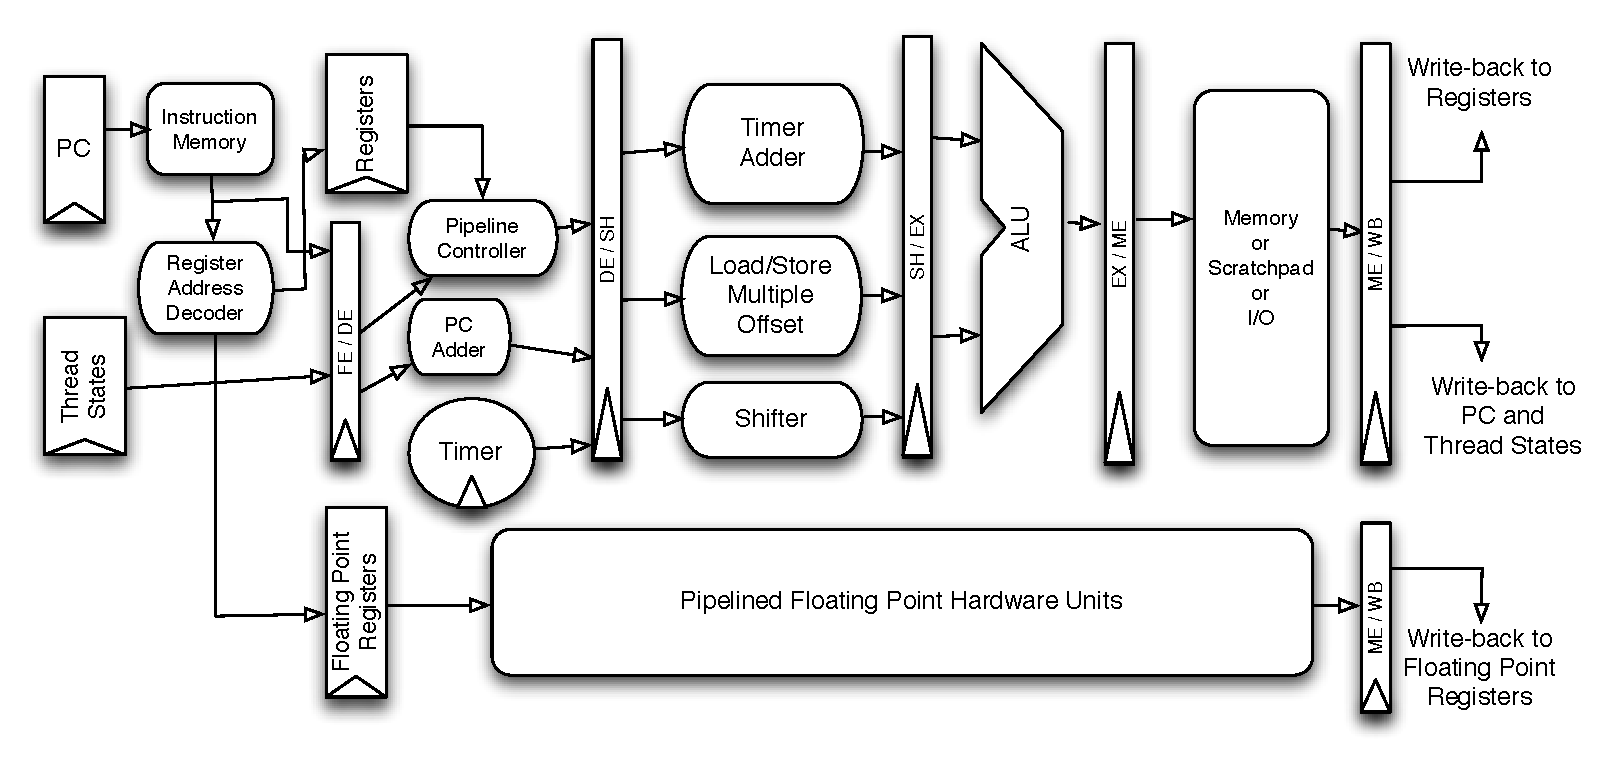
\includegraphics[scale=.54]{figs/ptarm_pipeline_six_stage}
  \end{center}
  \vspace{-20pt}
  \caption{The PTARM 6 Stage Pipeline}
  \label{fig:ptarm_pipeline_six_stage}
\end{figure}
This thread-interleaved pipeline follows the same design principles as discussed in chapter~\ref{chapter:pret}, and supports a minimum of six threads interleaved through the pipeline.
The memory footprint for each of the computational nodes range from roughly 100 to 1000 bytes.  
Thus, scratchpad memories are sufficient to hold all instructions and data for all threads within a PTARM core, no external memory is required. 
The pipeline also contains hardware floating point units to support the applications needs of floating point computations.
The floating point units are single-precision, and generated using the Xilinx Coregen tool~\cite{xilinx_coregen}. 
They are pipelined to accept input every cycle, which avoids structural hazards, as explained in section~\ref{section:pret_thread_pipeline}.   
The floating point operations supported are: add, subtract, multiply, float-to-fix, fix-to-float, divide and square root. 

Our pipeline design supports configurations which exclude certain floating point units, since not all computational nodes require all floating operations.   
For example, square root is only used by the valve node, and divide is only used by the ``T'' node, as shown in table~\ref{tab:1dcfd-inst-count}. 
The floating point divide and square root hardware are the most resource intensive units, but the valve and ``T'' nodes usually represent only a few percent of overall system.
The common fuel rail system we will present later contains 234 nodes, but only 5 nodes are ``T'' nodes and only 4 nodes are valves.
To save on hardware resources, we could use software emulation for the complex operations at the cost of increase the execution time of the ``T'' nodes and valve nodes.
However, the overall performance of our system is bounded by the slowest computational element, because all nodes synchronize communication points at the end of each time step.   
As a result, the performance hit from using software emulation for these small percent of nodes would limit the overall performance. 
Instead, by allowing different configurations of PTARM cores within the system, we can include the hardware additions only on cores that require them, getting the performance boost from hardware without a huge resource overhead.   
This results in substantial resource savings, which we show in section~\ref{sec:1dcfd-results}.

The real-time, highly parallel yet heterogeneous nature of this application makes it a perfect match for our Precision Timed Architecture.
As explained in section~\ref{section:pret_thread_pipeline}, thread-interleaved pipelines contain simpler pipeline architectures, allowing for higher clock frequencies and less resource usage.   
The sharing of the data-path between multiple hardware threads further allows us to optimize the resource usage per computational element.
%We discuss in more details the trade-offs involving adding threads later in section~\ref{sec:1dcfd-results}.
The thread-interleaved pipeline also maximizes throughput over latency, which benefits this highly parallel application.  
The pipeline hide the latencies of multi-cycle operations, such as floating point operations, with execution from other threads.
E.g., in our implementation, the normally 4 processor cycle floating-point additions and subtractions appear as single thread cycle instructions because their latencies are fully hidden by the thread interleaving. 

\paragraph{Interconnect}
\begin{wrapfigure}{r}{0.5\textwidth}
\centering
\includegraphics[page=8, width=0.49\textwidth]{./figs/1dcfd/FCCM2012Figures.pdf}
%\caption{System of Multi-threaded PRET Cores and Interconnects}
\caption{System of PRET Cores and Interconnects}
\label{fig:1dcfd-hardware}
\vspace{-5mm}
\end{wrapfigure} 
This application requires support for two types of communication.
Between neighboring nodes, the pressure and flow rate values computed are exchanged every time step.
Across the system, several temperature dependent parameters are calculated and broadcast to all nodes every time step as well.
Thus, along with point to point communications between nodes, we also implement a global broadcast circuit.     
Each node can receive up to four inputs and transmit four outputs each time step, depending on the number of neighboring nodes it is connected to.
Out of the inputs, one is dedicated to receiving broadcasts from the global distribution circuit.

Because nodes are mapped to hardware threads on a core, their neighboring node may be mapped to another thread on the same core, or a thread on a neighboring core.  
Nodes mapped to the same core (intra-core communication) communicate through the shared scratchpad memory within the core.
For nodes mapped to different cores (inter-core communication), we use privately shared Block RAMs (BRAMs) between cores to establish the point-to-point communication channel.
BRAMs are dedicated memories on the FPGA that provide single cycle deterministic access latencies, scratchpad memories within each core are also synthesized to BRAMs.
Because the communication bandwidth requirements are small, we only need one shared BRAM between two cores to establish communication channels for all threads on both cores.
This allows all threads to communicate with each other with single cycle latency, whether it is intra-core or inter-core communication.   
As an added benefit, by using BRAMs for communication, we save the logic slices on the FPGA to implement more cores to support bigger models.
On modern FPGAs, the limiting resource factor is typically logic slices, not BRAMs.
Each core only requires a small number of BRAMs to be used for registers and scratchpads, so the BRAM utilization ratio is far less than the logic slice utilization ratio when we synthesize many cores. 
As we present our synthesis results in section~\ref{sec:1dcfd-results}, we will show that the number of cores synthesized is indeed limited by the logic slices, not the BRAMs. 
 
When implementing the global distribution circuit, we observed that only a few nodes are required to the broadcast all the temperature dependent parameters.   
In fact, in diesel fuel systems, the number of nodes needed to broadcast all parameters can be mapped to the six threads of one single PTARM core. 
Thus, we dedicate one PTARM core in the system as the broadcast core.
For each other core, we add a dedicated broadcast receiving memory that is connected to the broadcast core.
The broadcast receiving memory is also synthesized to a small dual-port BRAM, with a read-only port connected to the core, and a write-only port connected to the broadcaster.
The broadcast core contains a broadcast bus that can simultaneously write to all the broadcast memories the same values.
The broadcast memory is also shared amongst all threads in a core so all threads can access the global values. 
This architecture allows us to save on the resources needed to implement a full fledged interconnect routing system or any network protocol to be used for broadcasting. 
Figure~\ref{fig:1dcfd-hardware} shows a block-level view of the hardware architecture.    

%------------------------------------------------------------------------ 
\subsubsection{Software Architecture}
\label{sec:1dcfd-software_architecture}
We implement the equations in table~\ref{tab:1dcfd_pipe_types} in the language C and compile it with the GNU ARM cross compiler~\cite{gnu-arm} to run on our cores. 
In order to minimize the computation required, the equations are statically optimized.  
%Table~\ref{tab:1dcfd-inst-count} show the number of multiply, add/subtract, absolute value, square root, and divide operations required by each computational node after optimization.
The communication channels in and out of each node is memory mapped to the shared BRAMs between cores.

The execution of the system progresses in time steps.  
Computational nodes have varying execution speeds, to avoid data races and ensure all communication is synchronized each time step, we enforce an execution model where each time step consists of several synchronized phases, as shown in figure~\ref{fig:1dcfd-software_model}.
For pipe nodes that read in neighboring data, shown on the top of figure~\ref{fig:1dcfd-software_model}, the first phase of each time step is to read in pressure and flow rate values from neighboring nodes, and the temperature dependent variables from the global broadcasters.
Once input values are read, the computation occurs according to the specific fluid dynamics equations.
The final phase of each time step, the computed results are posted to be used in the next time step.
For global and mechanical nodes, the two phases consists of reading in external values for calculation, and posting results.
We synchronize the data exchange between nodes to ensure avoid data races and ensure that all data operated on is consistent and from the same time step. 
This communication model is very similar to Giotto~\cite{henzinger_giotto}, where tasks communicate explicitly through ports, and only at the end of execution of the tasks to ensure deterministic communication between the tasks. 
While implementations of Giotto use an explicit run-time system to enforce the execution model, we use the timing instructions provided by the PRET architecture to implement our system.   

\begin{figure}
\centering
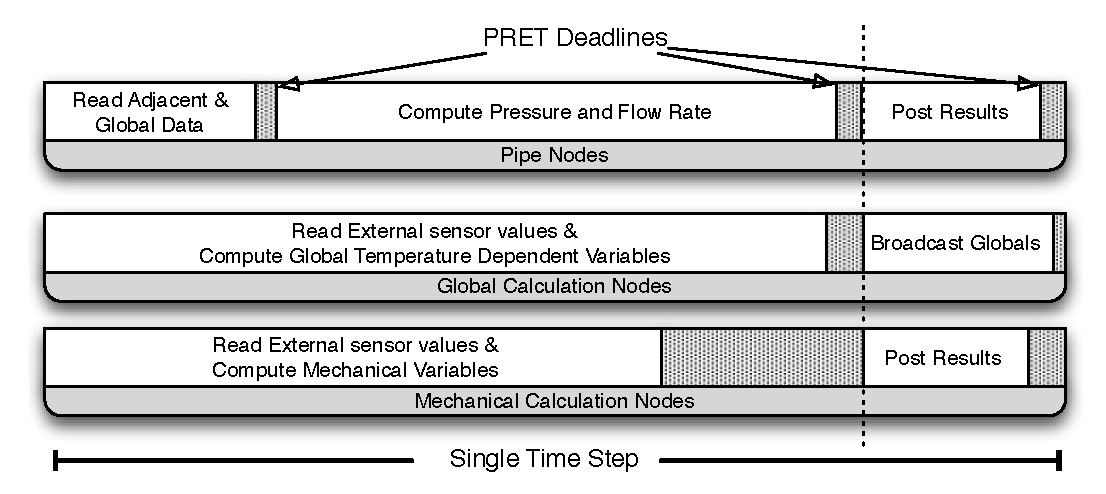
\includegraphics[scale=0.6]{./figs/1dcfd/software_execution_model.pdf}
\caption{Execution of Nodes at Each Time Step}
\label{fig:1dcfd-software_model}
\vspace{-5mm}
\end{figure}

In section~\ref{sec:programming_models} we introduced ISA extensions that provide programmers with explicit timing control in software.  
The implementation of the various timing instructions for PTARM is explained in section~\ref{sec:ptarm_instructions}.
Specifically for this application, we use a specialized timing macro \emph{delay\_and\_set}, which uses \delayuntil, as introduced in section~\ref{sec:programming_models}.
The semantics of the \emph{delay\_and\_set} instruction is similar to the deadline instruction introduced by Ip and Edwards~\cite{ip2006processor}. 
When it is decoded, it first enforces the previously specified timing constraint, then it sets a new timing constraint for the next code block. 
The instruction enforces a minimum execution time within the code, which we use to enforce the synchronized execution of time steps for all nodes.  
Fig.~\ref{fig:1dcfd-software_model} shows the program synchronization points that our timing instruction enforces.
The hatched area in the figure denotes slack time that is generated by the timing instructions.
Each \emph{delay\_and\_set} instruction takes 2 thread cycles because it manipulates a 64-bit value representing time. 
For our computational nodes, 3 timing instructions are used each time step, thus 6 thread cycles of overhead are introduced per time step.
%The overhead is already included in our execution time analysis presented in table~\ref{tab:1dcfd-inst-count}.

The timing instructions provide a very lightweight and simple mechanism to enforce synchronization in software.
No additional run-time system is needed to enforce the execution model, and we avoid the need to use locks or mutex to ensure correct ordering of communicated data. 
%Instead, on a timing predictable architecture, we use time to synchronize the execution all computational nodes.
The same effect can possibly be achieved with no overhead using instruction counting and NOP insertions.
This can certainly be done on any deterministic architecture such as PRET. 
However, NOP insertion is both brittle and tedious. 
Any change in the code would change the timing of the software and insertions need to be adjusted to ensure the correct number of NOPs are added.
Designs now are mostly written in programming languages like the language C and compiled into assembly, making it even more difficult to gauge the number of NOPs needed at design time.
The timing instructions allow for a much more scalable and flexible approach. 
In a system with heterogeneous nodes and different execution times, the timing instructions allow us to set the same timing constraints in all nodes regardless of its execution time.   

The \emph{delay\_and\_set} instruction only enforces minimum execution time, but does not guarantee that the worst-case execution time of all computational nodes meet the timing constraints imposed from the application.
Static timing analysis on all nodes is still required to verify that the worst-case execution time of time steps meets the imposed timing constraints by the application parameters.
However, as soon as the timing constraints are met, there are no additional benefits to improving the execution speed of the computational nodes.
As system time steps are synchronized with sensors that interface with the physical world, and execution is real-time along the engine. 
In this case, precise execution time analysis can help us optimize other system resources, such as power and area, improving the scalability of the approach.
On the other hand, over estimation of execution time could lead to over-provisioning of hardware resources.    
In this application, the computation code on the nodes within each time step contains only a single path of execution, voiding the need for complex software analysis.
Thus, the predictability of the underlying architecture determines how precise the worst-case execution time analysis is.
Communication is handled by the synchronized communication points, which enforces an ordering between the writing and reading of shared data.
This voids the need of any explicit synchronization methods, removing any overhead and unpredictability for communication.
The underlying architecture uses the time-predictable PRET, and implements a latency-deterministic communication network of shared BRAMs on the FPGA. 
These properties allow us to statically obtain an exact execution time for each computation node, which we will show and present in the next section. 

%------------------------------------------------------------------------ 
\subsection {Experimental Results and Discussion}
\label{sec:1dcfd-results}
We use three examples to evaluate our framework.
The first example is a simple waterhammer example taken from Wylie and Streeter~\cite{1978FluidTransients}.
It is similar to the one shown in figure~\ref{fig:1dcfd-DetailedDiagram}, but without the ``T" element and the nodes that branch up.
This example contains an imposed pressure, 5 pipe segments, a valve, and two mechanical input blocks that provide both the reference pressure and the valve angle as a function of time.
We use this simply as a sanity check for the correctness of functionality of our framework.
  
The second and third example cover two common diesel injector configurations: the unit pump and common rail.  
The data for configuring these cases was taken from reference examples provided by Gamma Technologies' GT-SUITE software package~\cite{GTFuel}. 
The unit pump is much like the simple waterhammer case in that there are no branches in the system.  
The input is a defined flow specified by an electronically controlled cam driven pump.  
The output is a single valve.  
There are a total of 73 fluid sub-volumes in this system. 
%
The common rail example is more complex where the topology is roughly that described by the 1D-CFD model in figure~\ref{fig:1dcfd-DetailedDiagram}.  
It has a total of 234 sub-volumes, including 5 ``T" intersections and 4 valves.
Both the GT-SUITE-based models use a 1 $cm$ discretization length, which, using a 1500 $m/s$ wave speed, and a stability factor of 0.8 yields a 5.33\(\mu s\) time step to complete our worst-case instructions for the slowest computational node.

We synthesize all our cores and interconnects on the Xilinx Virtex 6 xc6vlx195t~\cite{v6_manual} with speed grade 3.
Each Virtex-6 FPGA logic slice contains 4 LUTs and 8 flip-flops, and this FPGA contains 31,200 logic slices and 512 18-$KB$ BRAMs.
Each PRET core is clocked at 150 $MHz$ and has 6 threads.
All floating point units are generated from the Xilinx Coregen tool~\cite{xilinx_coregen}, and are configured to maximize DSP slice usage and minimize logic slice usage as much as possible.
We save the logic slices to synthesize as many cores as possible.
Our current PRET implementation, the PTARM, uses an ARM-based ISA, thus our C code is compiled using the GNU ARM cross compiler~\cite{gnu-arm} with the optimization compiler flag set to level 3.  
For these examples, we used a mapping heuristic that grouped nodes requiring same computations onto the same core. 
In the sections below we will show that this heuristic allows us to save hardware resources by synthesizing less floating point units. 

\subsubsection{Timing Requirements Validation}
In order to ensure that the worst-case computational element can meet the timing requirements, static timing analysis is done on all computational nodes to determine the worst-case execution of each time step.
As discussed in section~\ref{sec:1dcfd-software_architecture}, the computation code within each time step only consists of a single path, simplifying the timing analysis.
The thread-interleaved pipeline provides temporal isolation for all hardware threads, so no timing interference occurs between the threads.
We can safely use the timing analysis done separately for each computational node even as they are executed simultaneously in the architecture.
Because all code, data, and communication channels reside on the BRAMs of the FPGA, the access latency is all deterministically one cycle.
The PTARM architecture provides deterministic execution time for each instruction implemented, and the full list of instruction execution cycles is listed in table~\ref{table:ptarm_instruction_timing}.
Most floating point instructions take only a single thread cycle, as the latency is fully hidden by interleaving the hardware threads in the pipeline.
The more complex floating point square root and divide operations take four thread cycles.
Using the deterministic instruction execution cycles and the compiled code, we are able to obtain the exact thread cycles required for each computational node, which is shown in table~\ref{tab:1dcfd-inst-count}.  

\begin{table}
\begin{center}
\begin{smalltabular}{|l|c|c|c|c|c|c|}
\hline
 & \multicolumn{6}{c|}{Without Interpolation / With Interpolation} \\
\hline
Type	& Mul	& Add/Sub	& Abs	& Sqrt	&Div	&Thread cycles \\ 
\hline \hline
Pipe segment					&10 / 18	&5 / 13		&2 / 2		&0 / 0 		&0 / 0		&51 / 81 \\ 
\hline
Imposed pressure 						&6 / 10		&3 / 7		&1 / 1		&0 / 0 		&0 / 0		&38 / 50 \\ 
\hline
Imposed flow			&5 / 9		&3 / 7		&1 / 1		&0 / 0 		&0 / 0		&40 / 51\\ 
\hline
Valve 						&13 / 17	&5 / 9 		&1 / 1		&1 / 1 		&0 / 0		&55 / 64 \\ 
\hline
Cap 							&4 / 8		&2 / 6 		&1 / 1		&0 / 0 		&0 / 0		&39 / 48 \\ 
\hline
Pipe ``T" 		&16 / 28 	&13 / 25 		&3 / 0		&0 / 0 		&4 / 4		&72 / 111 \\ 
\hline  
\end{smalltabular}
\end{center}
\caption{Computational Intensity of Supported Types}
\label{tab:1dcfd-inst-count}
\vspace{-2mm}
\end{table}

%A hardware context switch occurs every processor cycle, and threads are scheduled in a round robin order.
To convert thread cycles to physical time, we use the processor clock speed and number of threads executing in the architecture. 
Given a 150~$MHz$ clock rate and six hardware threads, each thread executes at 25~$Mhz$ in our thread-interleaved pipeline. 
Thus, each thread cycle converted to physical time is 40~$ns$ long.
The unit pump and common rail have a requirement of 5.33~$\mu s$, which gives us 133 thread cycles to complete the computation each time step. 
Table~\ref{tab:1dcfd-inst-count} shows that the ``T'' element, which takes 111 thread cycles with interpolation, is the node with the worst-case execution time, well below the 133 thread cycle constraint. 
For the simple waterhammer example, a bigger discretization $\Delta x$ is used, which leads to a bigger time step than that of the two complex examples.
This validates that we can safely meet the timing requirements, ensuring the correctness of functionality of our implementation.   

\subsubsection{Resource Utilization}

Table~\ref{tab:1cfd-Cores_vs_features} shows the resource usage in logic slices for different configurations of a PTARM core.
Each core uses 7 BRAMs: 3 for the integer unit register set (3 read and 1 write port), 2 for floating point register set (2 read and 1 write port), 1 for the scratchpad, and 1 for the global broadcast receiving memory.
We include the fixed point configuration for reference purposes, as it doesn't contain any floating point units.
The baseline configuration used in our implementation is the ``basic float'', which contains a floating point add/subtracter, a floating point multiplier, and float to fix conversion units.
The ``sqrt'', ``div'' and ``sqrt \& div'' configurations add the corresponding hardware units onto the ``basic float'' configuration. 
Besides the effect of hardware units, we also show the area impact of adjusting the thread count on a single core.

\begin{table}[hbt!]
\begin{center}
\begin{tabular}{|l|c|c|c|c|c|c|}
\hline
Threads per core & 6 & 8 & 9 & 16\\ \hline\hline
Fixed point only  & 572 & 588 & 764 & 779\\ \hline
Basic float  & 820 & 823 & 1000 & 1022 \\ \hline
Float with sqrt  & 987 & 992 & 1146 & 1172 \\  \hline
Float with div  & 1039 & 1051 & 1231 & 1237 \\ \hline
Float with div \& sqrt  & 1237 & 1249 & 1403 & 1413 \\ \hline
\end{tabular}
\end{center}
\caption{Number of Occupied Slices per Core on the Virtex 6 (xc6vlx195t) FPGA.}
\label{tab:1cfd-Cores_vs_features}
\vspace{-2mm}
\end{table}

Two important observations are made from the results of table~\ref{tab:1cfd-Cores_vs_features}.
First, the area increase associated with adding more threads to the core is proportional only to the number of bits required to encode the number of threads.  
For example, running 6 threads or 8 threads (both requiring three bits to encode the thread number) on the processor yields a similar area usage.
But once a 9th thread is introduced, the used area noticeably increases, but remains similar for up to 16 threads. 
This can be explained by understanding the architecture of multi-threaded processors. 
Multi-threaded processors maintain independent register sets and processor states for each thread, while sharing the datapath and ALU units amongst all threads.
The register sets are synthesized onto BRAMs, so the number of bits used to encode thread IDs will determine how big of a BRAM is used for the register set. 
The size of the multiplexers used to select thread states and registers is also determined by the number of bits encoding the thread IDs, not the actual number of threads running. 
Thus, it is possible to increase the number of threads per core with almost negligible impact on area as long as the incremented thread count uses the same number of bits to encode.    
Increasing the thread capacities will allow our architecture to support more nodes in a single FPGA.
However, since hardware threads share the processor pipeline, adding threads slows down the running speed of the individual threads.
Nonetheless, for implementation that have sufficient slack time or require faster performance, adjusting the number of threads could lead to a valuable improvement.
Our precise execution time analysis allows us to determine the maximum number of threads, six in our case, we can support to meet our timing constraints.
An over estimated execution time in this case could lead to under utilizing the hardware by constraining the number of threads to five, resulting in requiring additional cores to implement our 237 node fuel rail example.     

The second observation relates to the resource impact of the floating point square root and divide units. 
Looking at the resource usage for 6 threads on a core, adding a floating point square root unit adds roughly 20.3\% more logic slices than the ``basic float'' configuration.  
Ading a floating point division unit adds roughly 26.7\% more logic slices than the ``basic float" configuration.  
A core with both square root and division unit would use roughly 50.8\% more slices.
These are estimates because the slices occupied might vary slightly based on how the synthesis tool maps LUTs and flip flops to logic slices. 
But they give an intuition to the resource difference used for each configuration.

The actual resource impact can be seen from Table~\ref{table:1dcfd-example_results}, which shows the total slices occupied when the three examples we implemented are synthesized.
In the homogeneous (hom. suffix) configuration, all the cores contain the square root and divide hardware.
In the heterogeneous (het. suffix) configuration, only necessary cores contain square root and divide, the rest use the basic float configuration.  

\begin{table}[htb!]
\vspace{-2mm}
\begin{center}
\begin{smalltabular}{|c|c|c|c|c|c|c|c|}
\hline
\multicolumn{2}{|c}{\multirow{2}{*}{Example}}	& \multicolumn{1}{|@{\hspace{0.5mm}}c@{\hspace{0.5mm}}|}{\multirow{2}{*}{Nodes}}	& \multicolumn{1}{|@{\hspace{0.5mm}}c@{\hspace{0.5mm}}|}{\multirow{2}{*}{Cores / Conn.}}	& \multicolumn{2}{|c|}{Slices / BRAM}  \\
\cline{5-6}
\multicolumn{2}{|c|}{}	&	&	& Absolute	& \multicolumn{1}{|@{\hspace{1mm}}c@{\hspace{1mm}}|}{Relative (\%)}	\\ 
\hline\hline
Water	& het.	& \multirow{2}{*}{12}	& \multirow{2}{*}{2 / 1}	& 1805 / 15	& 5.7 / 2.1 \\ 
\cline{2-2}\cline{5-6}
Hammer	& \multicolumn{1}{|@{\hspace{1mm}}c@{\hspace{1mm}}|}{hom.}	&	&	& 2379 / 15	& 7.6 / 2.1\\ 
\hline
Unit	& het.	& \multirow{2}{*}{73}	& \multirow{2}{*}{13 / 12}	& 10566 / 103	& 33.0 / 15.0\\ 
\cline{2-2}\cline{5-6}
Pump	& hom.	&	&	& 16635 / 103	& 44.0 / 15.0\\ 
\hline
\multicolumn{1}{|@{\hspace{1mm}}c@{\hspace{1mm}}|}{Common}	& het.	& \multirow{2}{*}{234}	& \multirow{2}{*}{39 / 38}	& \multicolumn{1}{|@{\hspace{1mm}}c@{\hspace{1mm}}|}{29134 / 311}	& 93.4 / 45.0 \\ 
\cline{2-2}\cline{5-6}
Rail	& hom.	&	&	& \multicolumn{2}{c|}{N/A} \\ 
\hline
\end{smalltabular}
\end{center}
\caption{Total Resource Utilization of Examples Synthesized on the Virtex 6 (xc6vlx195t) FPGA}
\label{table:1dcfd-example_results}
\vspace{-2mm}
\end{table}

For the simple waterhammer example, since only 2 cores are used, the savings is less noticeable. 
But as the application size scales up, the resource savings of a heterogeneous architecture become more apparent.
The homogeneous approach uses roughly 1.5 times the number of slices our heterogeneous approach uses, which is consistent with the findings in table~\ref{tab:1cfd-Cores_vs_features}.
This proved to be critical for the 234-node common rail example, as only our heterogeneous architecture could implement the design on the xc6vlx195t FPGA while the homogeneous design simply could not fit.
These results also reflect our decision to use a heuristic that groups nodes with the similar computation together. 
By doing so, we can synthesize less hardware floating point units overall, saving hardware resources.
Table~\ref{table:1dcfd-example_results} also shows the BRAM usage for the implemented examples. 
Each interconnect uses 1 BRAM and each core uses 7 BRAMs. 
We see that the BRAM utilization ratio is far below the logic cell utilization, validating our design choice of using BRAMs for interconnects and broadcasts.     

%-------------------------------------------------------------------------
\subsection{Conclusion}
%\todo{add more explanation of why this app is important for PRET}
In this application, we presented a novel framework for solving a class of heterogeneous micro-parallel problems.  
Specifically we showed that our approach is sufficient to model a diesel fuel system in real time using the 1D-CFD approach on FPGAs.
To the best of our knowledge, we believe this is the first attempt to attack real-time CFD on this timescale and complexity of problem.
There may exist different implementation options for our application on FPGAs. 
For example, we could attempt the problem in discrete FPGA blocks.  
However, in order to make the application fit in a practical FPGA, we would need to re-use the hardware multipliers, adders, and other functional units.  
This would require a state machine to run it and begins to look a great deal like a processor.

Instead, we use the PRET architecture to ensure timing determinism and implement a light-weight timing based synchronization on a multicore PRET architecture.
We set up a configurable heterogeneous architecture that leverages the programmability of FPGAs to efficiently synthesize the design for efficient area usage. 
Our results show ample resource savings, proving that our approach is practical and scalable to larger and more complex systems.

%	It is important to understand that in our framework, 
	%PRET timing instructions are used to enforce the periodic behavior of the application, while the precise timing analysis allows us to ensure that the timing requirements are met. 
	%Communication and synchronization of the cores are timing based, thus adding cores or threads does not add any overhead or affect performance.

%We plan to continue to extend this work along several lines.  
%From the application perspective, we continue to add more flow element types to our library and compare our results to more complex flow systems.  
%We also plan to examine more closely the integration of mechanical and electrical nodes in our library.
%For the hardware architecture, we can to explore multi-rate timing of nodes to allow for differences in electrical, fluid, and mechanical timesteps.  
%
